\begin{center}
	\Large\textbf{\MakeUppercase{Программирование RISC-V}}
\end{center}

\section{Постановка задачи}
\begin{enumerate}
	\item Изучить методические материалы, доступные на сайте курса.
	\item Разработать программу на языке ассемблера RISC-V, реализующую определенную вариантом задания функциональность, отладить программу в симуляторе VSim/Jupiter. Массив (массивы) данных и другие параметры (преобразуемое число, длина массива, параметр статистики и пр.) располагаются в памяти по фиксированным адресам.
	\item Выделить определенную вариантом задания функциональность в подпрограмму, организованную в соответствии с ABI, разработать использующую ее тестовую программу. Адрес обрабатываемого массива данных и другие значения передавать через параметры подпрограммы в соответствии с ABI. Тестовая программа должна состоять из инициализирующего кода, кода завершения, подпрограммы main и тестируемой подпрограммы.
\end{enumerate}

\section{Вариант задания}
6) Определение медианы in-place.

\newpage

\section{Реализация на языке С}

Перед началом разработки данной по варианту программы на языке ассемблера RISC-V, был написан код на языке программирования C, выполняющий функции, требуемые в задании: ищет медиану в данном массиве:

\begin{code}
	\inputminted[breaklines=true, xleftmargin=1em, linenos, frame=single, framesep=10pt, fontsize=\footnotesize, firstline=1, lastline=33]{c}{listings/median.c}
	\caption{Код для нахождения медианы массива на языке С}
\end{code}

Данный код будет использован в качестве опоры для написания кода на языке ассемблера RISC-V

\section{Программа на языке ассемблера RISC-V}

\subsection{Код программы}
Данная по варианту функциональность была реализована на языке ассемблера RISC-V в виде единой программы. Код программы представлен на листинге 2.

\begin{code}
	\inputminted[breaklines=true, xleftmargin=1em, linenos, frame=single, framesep=10pt, fontsize=\footnotesize, firstline=1]{asm}{listings/full/median_full.s}
	\caption{Код для нахождения медианы массива на языке ассемблера RISC-V}
\end{code}

\subsection{Входные данные}

\begin{itemize}
	\item В секции \(.data\) задан исходный массив \(array = [10, 30, 56, 79, 47, 90, 100, 101]\).
	\item В секции \(.rodata\) (секция неизменяемых данных/констант) указан размер названного ранее массива, в данном случае \(n = 8\).
\end{itemize}

\subsection{Результат работы программы}
В результате работы программы происходит сортировка пузырьком исходного массива \(array\), сортированный массив будет находиться в тех же адресах, где и был исходный (сортировка in-place). После чего происходит нахождение медианы в зависимости от четности размерности массива и выводится в консоль симулятора.

Результат выполнения программы представлен на рис. 4.1.

\begin{figure}[H]
	\centering
	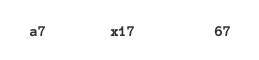
\includegraphics[]{riscv-result.png}
	\caption{Результат выполнения программы}
\end{figure}

Сравним результат с полученным значением при выполнении программы, написанной на языке C.

\begin{figure}[H]
	\centering
	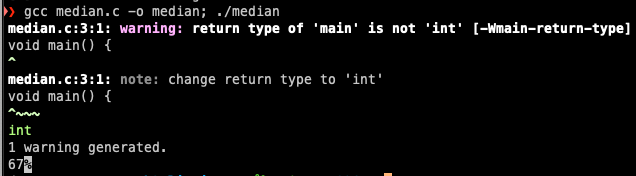
\includegraphics[width=15cm]{c-result.png}
	\caption{Результат выполнения программы на С}
\end{figure}

\subsection{Правила работы с программой}
\begin{itemize}
	\item Размер массива записывается в секции \(.rodata\) в регистр \(n\)
	\item Элементы массива записываются в секции \(.data\) в регистр \(array\) через запятую
	\item Производится сборка файла \(median\_full.s\) и исполнение программного кода.
	\item Результат работы программы будет выведен в консоль симулятора.
\end{itemize}

\subsection{Вывод}
Результат выполнения программы RISC-V полностью соответствует ожидаемому, программа работает исправно.

\newpage

\section{Программа на языке ассемблера RISC-V с подпрограммой}

\subsection{Код программы}
В отличие от единой программы здесь программа состоит из нескольких файлов.
\begin{itemize}
	\item setup.s - вспомогательная программа, в которой находится первичная инструкция \(\_\_start\) и инструкция окончания выполнения \(finish\).
	\item main.s - основная программа, вызывающая подпрограммы. Здесь также записываются входные данные.
	\item median.s - подпрограмма, которая находит медиану массива.
	\item bubble\_sort.s - подпрограмма, выполняющая сортировку массива пузырьком.
\end{itemize}

Код программы и подпрограмм представлен на листингах 3-6.

\begin{code}
	\inputminted[breaklines=true, xleftmargin=1em, linenos, frame=single, framesep=10pt, fontsize=\footnotesize, firstline=1]{asm}{listings/setup.s}
	\caption{Код вспомогательной программы setup.s}
\end{code}

\begin{code}
	\inputminted[breaklines=true, xleftmargin=1em, linenos, frame=single, framesep=10pt, fontsize=\footnotesize, firstline=1]{asm}{listings/main.s}
	\caption{Код программы main.s}
\end{code}

\begin{code}
	\inputminted[breaklines=true, xleftmargin=1em, linenos, frame=single, framesep=10pt, fontsize=\footnotesize, firstline=1]{asm}{listings/bubble_sort.s}
	\caption{Код подпрограммы bubble\_sort.s}
\end{code}

\begin{code}
	\inputminted[breaklines=true, xleftmargin=1em, linenos, frame=single, framesep=10pt, fontsize=\footnotesize, firstline=1]{asm}{listings/median.s}
	\caption{Код подпрограммы median.s}
\end{code}

\subsection{Входные данные}

\begin{itemize}
	\item В секции \(.data\) в программе \(main\) задан исходный массив \(array = [10, 30, 56, 79, 47, 90, 100, 101]\).
	\item В секции \(.rodata\) (секция неизменяемых данных/констант) в программе \(main\) указан размер названного ранее массива, в данном случае \(n = 8\).
\end{itemize}

\subsection{Результат работы программы}
В результате работы программы происходит вызов подпрограммы \(bubble\_sort\), где происходит сортировка пузырьком исходного массива \(array\), сортированный массив будет находиться в тех же адресах, где и был исходный (сортировка in-place). После чего машина возвращается в программу \(main\), где происходит вызов подпрограммы \(median\), где происходит уже непосредственно нахождение медианы в зависимости от четности размерности массива и выводится в консоль симулятора.

Результат выполнения программы представлен на рис. 5.1.

\begin{figure}[H]
	\centering
	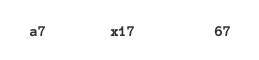
\includegraphics[]{riscv-result.png}
	\caption{Результат выполнения программы}
\end{figure}

Как можно заметить, результат полностью совпадает с программой, состоящей из одной программы.

\subsection{Правила работы с программой}
\begin{itemize}
	\item Размер массива записывается в секции \(.rodata\) в регистр \(n\)
	\item Элементы массива записываются в секции \(.data\) в регистр \(array\) через запятую
	\item Производится сборка файлов \(setup.s\), \(main.s\), \(bubble\_sort.s\), \(median.s\) и исполнение программного кода.
	\item Результат работы программы будет выведен в консоль симулятора.
\end{itemize}

\subsection{Вывод}
Результат выполнения программы RISC-V с подпрограммами полностью соответствует ожидаемому, программа работает исправно.

\section{Вывод по лабораторной работе}
В ходе выполнения работы было произведено ознакомление с архитектурой RISC-V и программированием на языке ассемблера этой архитектуры. Был реализован функционал нахождения медианы массива in-place в виде программы на языке ассемблера RISC-V и в виде программы с подпрограммами. Созданные в ходе работы программы работают полностью исправно.